\documentclass[a4paper,12pt,oneside]{article}

\usepackage{tikz}
\usetikzlibrary{positioning, shapes.geometric}
\definecolor{mycolor}{HTML}{FF5733}

\begin{document}
    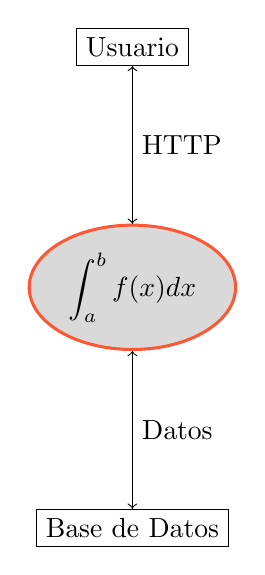
\begin{tikzpicture}[node distance=2cm, auto,
        % Definición de estilo para los nodos
        mynode/.style={
            draw=mycolor, 
            line width=1.1pt,
            ellipse, 
            fill=gray!30, 
            minimum width=2cm, 
            minimum height=1.5cm, 
            align=center
        }
    ]

        % Nodes
        \node[mynode] (server) {$\displaystyle \int_a^bf(x)dx$};
        \node[draw, rectangle, below=of server] (database) {Base de Datos};
        \node[draw, rectangle, above=of server] (user) {Usuario};
    
        % Lines
        \draw[->] (user) -- node {HTTP} (server);
        \draw[->] (server) -- node {} (database);
        \draw[->] (database) -- node[swap] {Datos} (server);
        \draw[->] (server) -- node[swap] {} (user);
    
    \end{tikzpicture}
  \end{document}